\section{Basics}
While \src{Common} is a layer atop of \src{Core}, \src{Common} itself consists of three more layers: \src{common}, \src{facile} and \src{support} (in their respective packages). The \src{facile} layer mostly contains stand-alone abstractions of classes/interfaces of \src{Core}, the \src{common} layer brings these abstractions together. The \src{support} layer contains exactly what it's name suggest: small, generic classes and methods that do not fit anywhere but that are really helpful in building up the other layers.

Clients almost exclusively have to make use of the \src{common} layer. They can use the other layers, but it seldomly makes sense to do so.

\subsection{Concepts}
In the understanding of \src{Common} an application consists of one main-window and maybe several supportive frames and dialogs. The main-window is most times a \src{JFrame} and the application runs as long as this frame is visible. The main-window consists of several panels, each showing some part of the data. E.g. the panels of a web-browser could be the ``history'', the ``bookmarks'' and the open websites.

\src{Common} adds an additional layer between panels and main-frame, it separates them and allows the user to drag \& drop panels. For this to happen the client needs to wrap each panel into a \src{CDockable}. These \src{CDockable}s are put onto a set of \src{CStation}s, a controller (of type \src{CControl}) manages the look, position, behavior etc. of all these elements. 

\begin{figure}[ht]
\centering
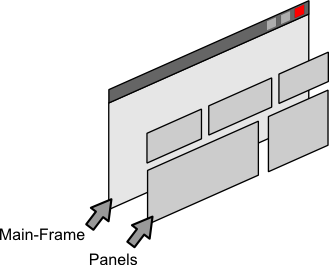
\includegraphics[scale=1]{basics/app_without}
\caption{The standard application without \src{Common}. A main-frame and some panels that are put onto the main-frame.}
\label{fig:app_without}
\end{figure}

\begin{figure}[ht]
\centering
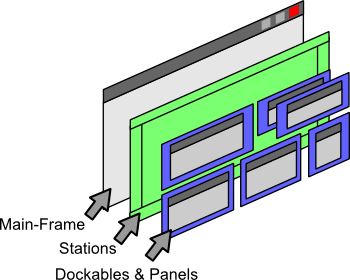
\includegraphics[scale=1]{basics/app_with}
\caption{An application with \src{Common}. The panels are wrapped into dockables. The dockables are put onto stations which lay on the main-frame. Dockables can be moved to different stations.}
\label{fig:app_with}
\end{figure}

\subsection{Hello World}
A first example containing only three colored panels will introduce the very basic vocabulary. In depth discussions of the concepts and implementations follow in the chapters afterwards.

\subsubsection{Setup controller}
The first step should be to create a \src{CControl}. This central controller wires all the objects of the framework together. A \src{CControl} needs to know the root window of the application, it is used as parent for any dialog that may be opened (e.g. during a drag \& drop operation a dialog may be used to paint the dragged element). Most applications will be able to just forward their root window to one the constructors of \src{CControl}.

The code to create the controller looks like this:
\begin{lstlisting}
public class Example{
	public static void main( String[] args ){
		JFrame frame = new JFrame();
		frame.setDefaultCloseOperation( JFrame.EXIT_ON_CLOSE );
		
		CControl control = new CControl( frame );
		
		...
\end{lstlisting}

\subsubsection{Setup stations}
The second step is to setup the layer between main-frame and dockables. There are different \src{CStation}s available. For example the \src{CMinimizeArea} shows minimized \src{CDockable}s. Instead of creating the stations manually one can also use a \src{CContentArea}. The \src{CContentArea} is a panel that consists of five stations. In the center a grid of dockables is shown, at the border four areas are reserved for minimized dockables.

There is always a default-\src{CContentArea} available, it can be accessed by calling \src{getContentArea} of \src{CControl}. If required additional \src{CContentArea}s can be created by the method \src{createContentArea} of \src{CControl}.

A \src{CContentArea} is a \src{JComponent}, so its usage is straight forward. Line \src{10} is the important new line in this code:
\begin{lstlisting}
public class Example{
	public static void main( String[] args ){
		JFrame frame = new JFrame();
		
		frame.setDefaultCloseOperation( JFrame.EXIT_ON_CLOSE );
		
		CControl control = new CControl( frame );
		
		frame.setLayout( new GridLayout( 1, 1 ) );
		frame.add( control.getContentArea() );
		
		...
\end{lstlisting}

\infobox{\src{CControl} always creates an additional station for handling externalized dockables.}

\subsubsection{Setup dockables}
The last step is to set up some \src{CDockable}s. \src{CDockable}s are the things that can be dragged and dropped by the user. A \src{CDockable} has a set of properties, e.g. what text to show as title, whether it can be maximized, what font to use when focused, and so on.
\src{CDockable}s are divided into two categories: ``single'' and ``multi'' dockables. These categories are explained later, for this first example single dockables are the correct choice. Single dockables are represented by the interface \src{SingleCDockable}. The class \src{DefaultSingleCDockable} provides an easy to use implementation.
In the code below new single dockables are created in lines \src{23-25} and \src{43-48}. They need to be registered at the \src{CControl} in lines \src{27-29}, otherwise they cannot be shown. Optionally the initial position can be set like in line \src{33} and \src{36}. There is no need to set the position of the first dockable \src{red}: since it is the first it gets per default all the space.

\begin{lstlisting}
import java.awt.Color;
import java.awt.GridLayout;

import javax.swing.JFrame;
import javax.swing.JPanel;

import bibliothek.gui.dock.common.CControl;
import bibliothek.gui.dock.common.CLocation;
import bibliothek.gui.dock.common.DefaultSingleCDockable;
import bibliothek.gui.dock.common.SingleCDockable;

public class Example{
	public static void main( String[] args ){
		JFrame frame = new JFrame();
		
		frame.setDefaultCloseOperation( JFrame.EXIT_ON_CLOSE );
		
		CControl control = new CControl( frame );
		
		frame.setLayout( new GridLayout( 1, 1 ) );
		frame.add( control.getContentArea() );
		
		SingleCDockable red = create( "Red", Color.RED );
		SingleCDockable green = create( "Green", Color.GREEN );
		SingleCDockable blue = create( "Blue", Color.BLUE );
		
		control.add( red );
		control.add( green );
		control.add( blue );
		
		red.setVisible( true );
		
		green.setLocation( CLocation.base().normalSouth( 0.4 ));
		green.setVisible( true );
		
		blue.setLocation( CLocation.base().normalEast( 0.3 ) );
		blue.setVisible( true );
		
		frame.setBounds( 20, 20, 400, 400 );
		frame.setVisible( true );
	}
	
	public static SingleCDockable create( String title, Color color ){
		JPanel background = new JPanel();
		background.setOpaque( true );
		background.setBackground( color );
		
		return new DefaultSingleCDockable( title, title, background );
	}
}

\end{lstlisting} 
